\documentclass{report}
\usepackage{tocloft}
\usepackage{geometry}
\usepackage{graphicx}
\usepackage{caption}
\usepackage[T1]{fontenc}
\usepackage[utf8]{inputenc}
\usepackage[polish]{babel}
\usepackage{float}
\usepackage{listings}
\usepackage{xcolor}

\geometry{
    a4paper,
    left=2.5cm,
    right=2.5cm,
    top=2.5cm,
    bottom=2.5cm,
}


\setcounter{tocdepth}{3}
\setlength{\cftbeforechapskip}{15pt} 
\setlength{\cftbeforesecskip}{8pt} 
\setlength{\cftbeforesubsecskip}{5pt} 
\setlength{\cftbeforesubsubsecskip}{5pt}

\renewcommand\thesection{\arabic{section}.}
\renewcommand\thesubsection{\thesection\arabic{subsection}.}
\renewcommand\thesubsubsection{\thesubsection\arabic{subsubsection}.}
\setcounter{secnumdepth}{3}


\begin{document}


\begin{titlepage}
    \centering
    \vspace*{1cm}
    \begin{figure}
        \centering 
        
\includegraphics[width=0.5\textwidth]{src/logo.png}
    \end{figure}
    \Huge
    Przemysłowe Bazy Danych
    \par
    
    \vspace*{1cm}

    \vspace{0.5cm}
    \LARGE \textit{Aplikacja testująca szybkość zapisu do plików tekstowych oraz bazy danych MS SQL Server}
    
    \vspace{1.5cm}
    
    \textbf{Autorzy:} 
    \par
    Jakub Pająk
    \par
    Kacper Stiborski
    \vspace*{1.5cm}
    \par AiR Grupa 5TI
    
    \vfill
    
    \Large Gliwice 2024 

\end{titlepage}

\newpage

\tableofcontents

\newpage

\section{\LARGE Wprowadzenie}
\subsection{\Large Cel projektu}

Celem projektu była implementacja aplikacji desktopowej, której zadaniem było wykonywanie operacji na plikach tekstowych oraz bazie danych. Aplikacja miała umożliwiać zapis określonej przez użytkownika liczby rekordów do pliku tekstowego oraz ich odczyt, a także dokonywać pomiaru czasu niezbędnego do wykonania tych operacji. Dodatkowo, projekt zakładał realizację analogicznych operacji na bazie danych MS SQL Server, z uwzględnieniem zapisu i odczytu rekordów oraz pomiaru wydajności obu procesów. Celem porównania efektywności operacji na plikach oraz bazie danych, aplikacja miała dostarczyć użytkownikowi czytelne informacje o czasie trwania poszczególnych zadań.


\section{\LARGE Realizacja projektu}

\subsection{\Large Interfejs użytkownika}

Interfejs użytkownika został zaprojektowany przy użyciu wbudowanego projektanta graficznego, będącego częścią frameworka \textit{Windows Forms}. Proces ten polegał na wybieraniu z przybornika (ang. \textit{Toolbox}) odpowiednich elementów funkcjonalnych, takich jak przyciski, etykiety czy pola tekstowe, i umieszczaniu ich na obszarze roboczym okna aplikacji. Dzięki narzędziu \textit{Properties}, możliwe było szczegółowe dostosowanie wyglądu i zachowania poszczególnych kontrolek do specyficznych wymagań projektowych, takich jak rozmiar, położenie, czcionka, czy reakcje na zdarzenia użytkownika.

\begin{figure}
    \centering
    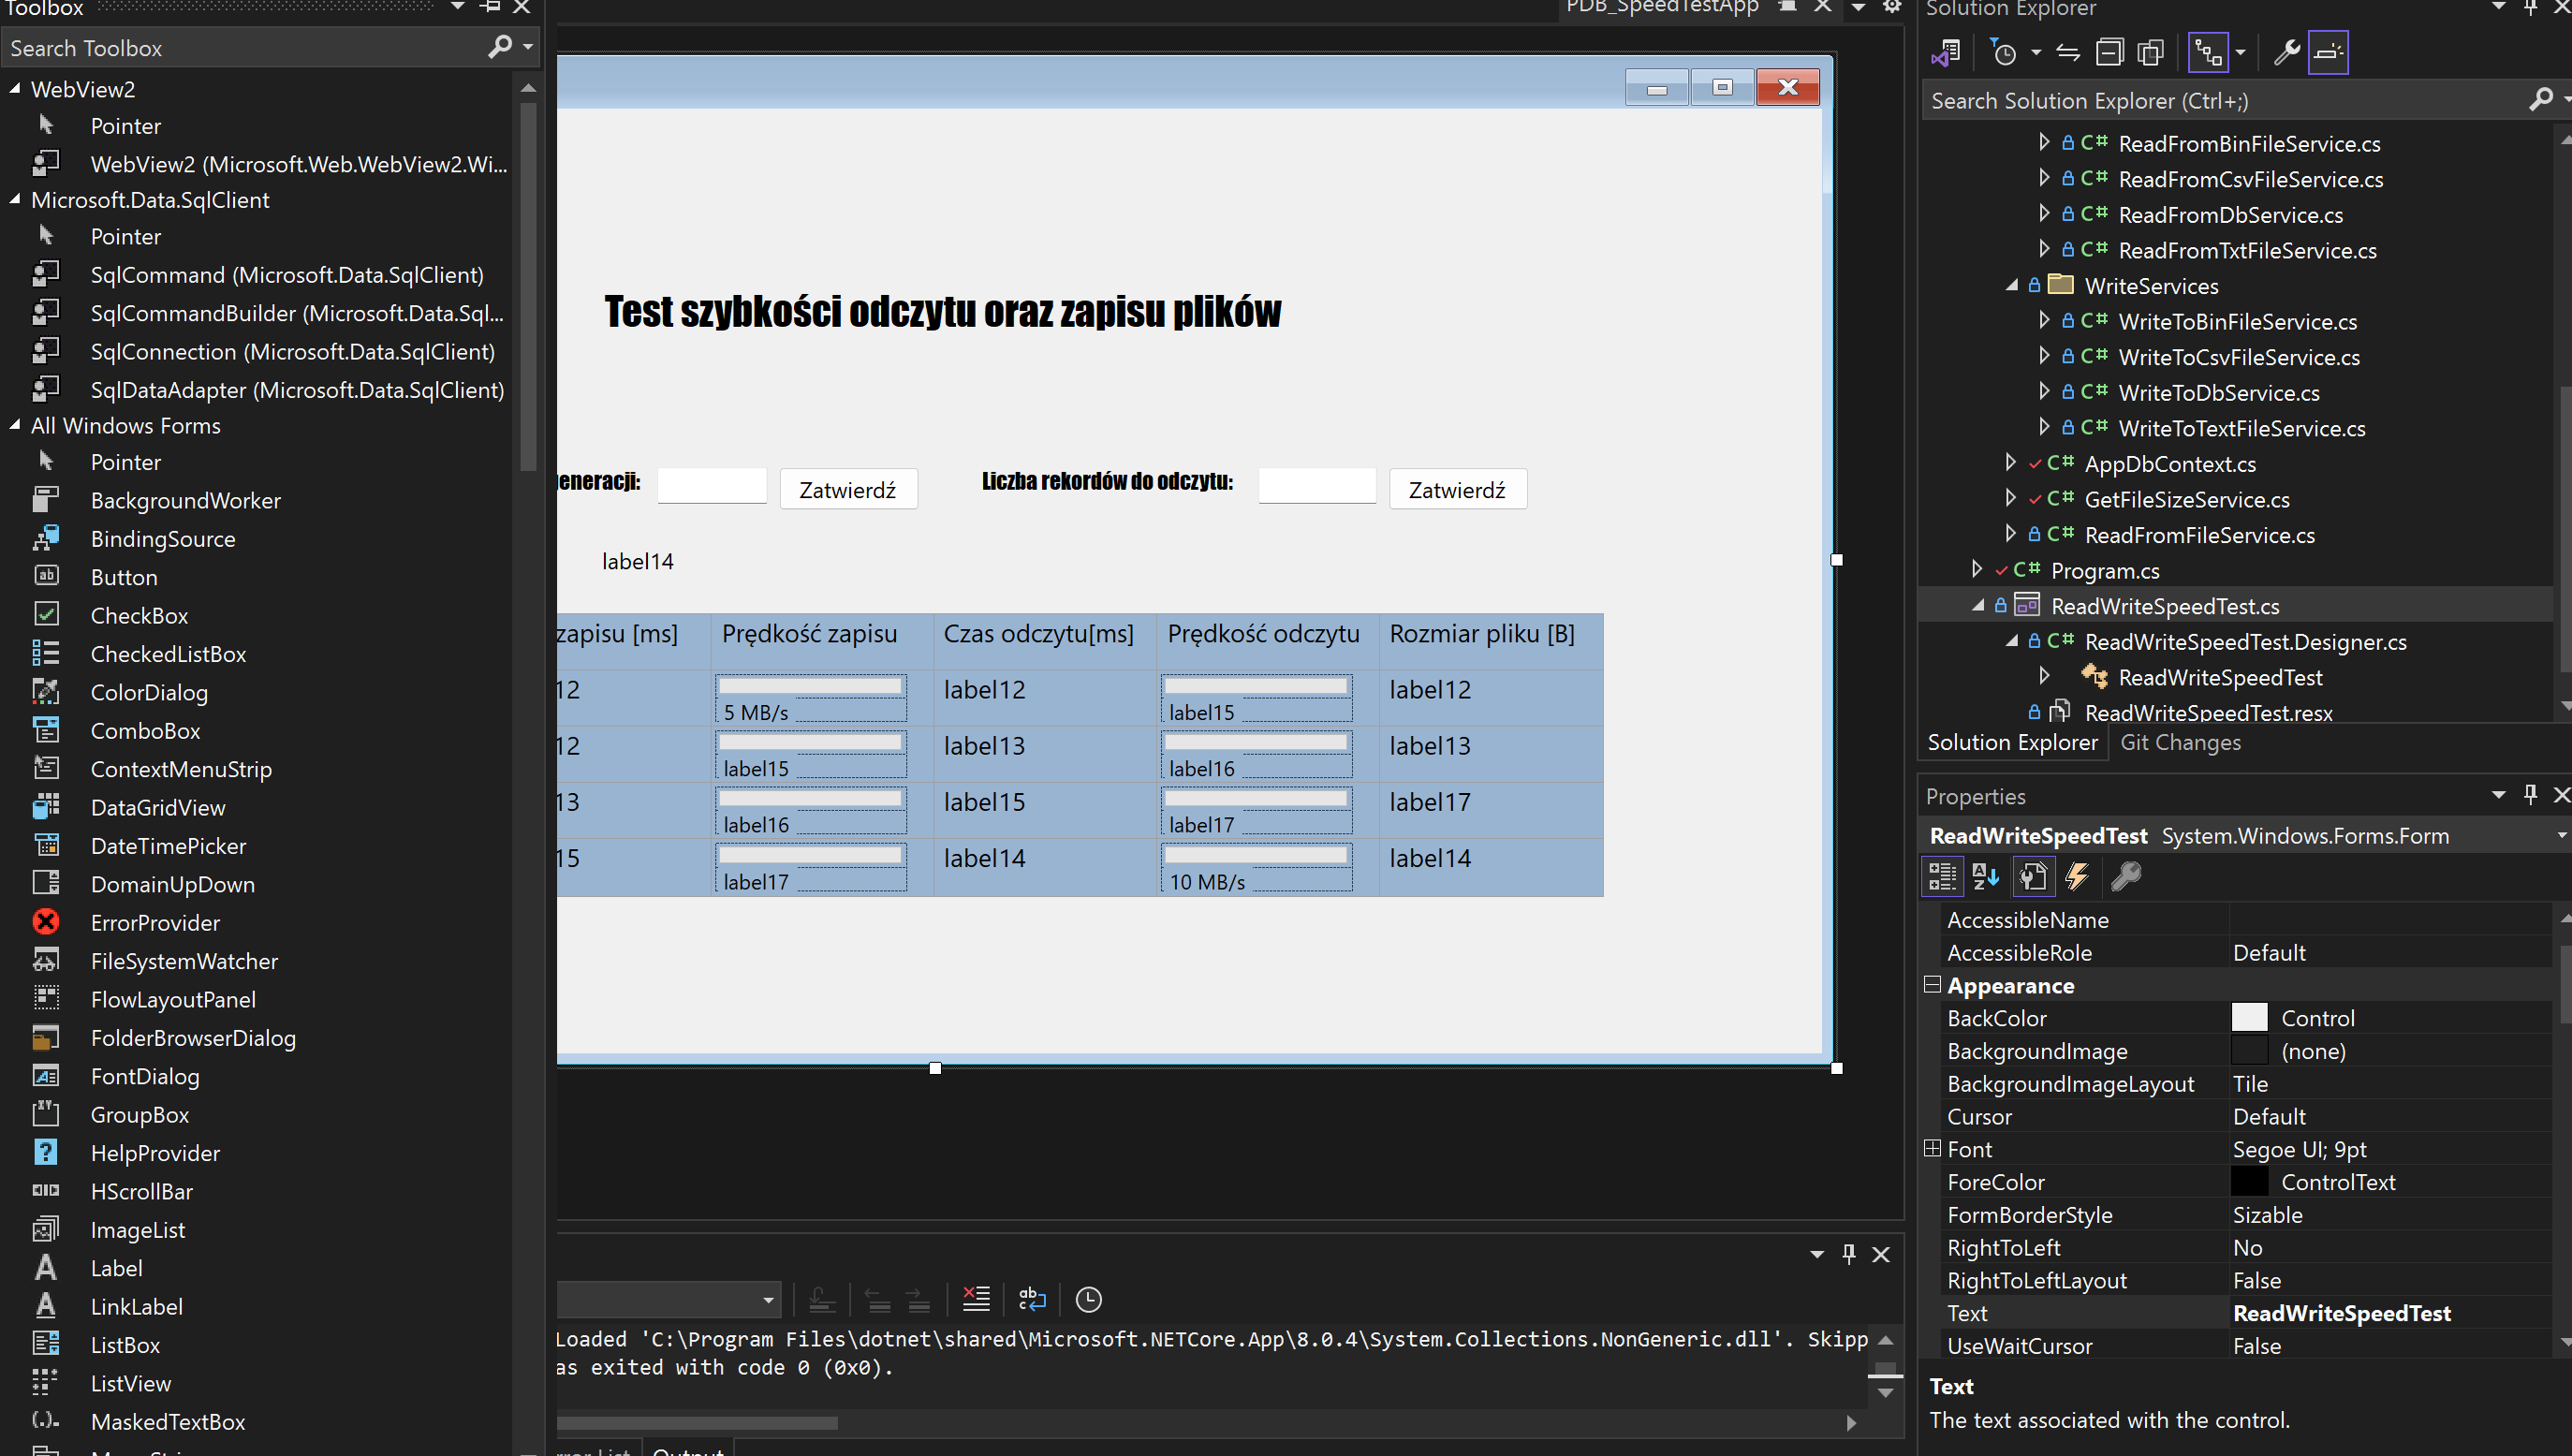
\includegraphics[width=1.0\textwidth]{src/interface-proj.png}
    \caption{Widok projektanta Windows Forms w IDE Visual Studio 2022}
\end{figure}


\subsection{\Large Obsługa zdarzeń i logika aplikacji}

Funkcja odpowiedzialna za inicjalizację oraz obsługę zdarzeń na głównym widoku aplikacji ma prostą, lecz efektywną strukturę. W konstruktorze następuje inicjalizacja widoku oraz przypisanie wartości początkowych zmiennym niezbędnym do działania aplikacji. Wszystkie kolejne funkcje związane z obsługą zdarzeń są generowane automatycznie przez Visual Studio, na przykład poprzez dwukrotne kliknięcie na kontrolkę w widoku projektanta. Tak właśnie zrealizowano obsługę przycisków w opisywanej aplikacji.

Główna funkcja logiki aplikacji wywołuje dwie metody pomocnicze: \textit{InvokeWriteServices()} oraz \textit{InvokeReadServices()}. Metody te z kolei korzystają z odpowiednich klas, które obsługują zapis i odczyt danych, zwracając wyniki w postaci zmiennej typu \textit{Dictionary<string, double>}. Klucz typu \textit{string} odpowiada za identyfikację typu pliku, natomiast wartość typu \textit{double} przechowuje czas potrzebny na wykonanie operacji.

Następnie, czasy operacji są przypisywane do obiektów typu \textit{Label}, co pozwala na ich wyświetlenie w interfejsie użytkownika, dostarczając czytelne informacje o wydajności działania aplikacji.

\begin{figure}
    \centering
    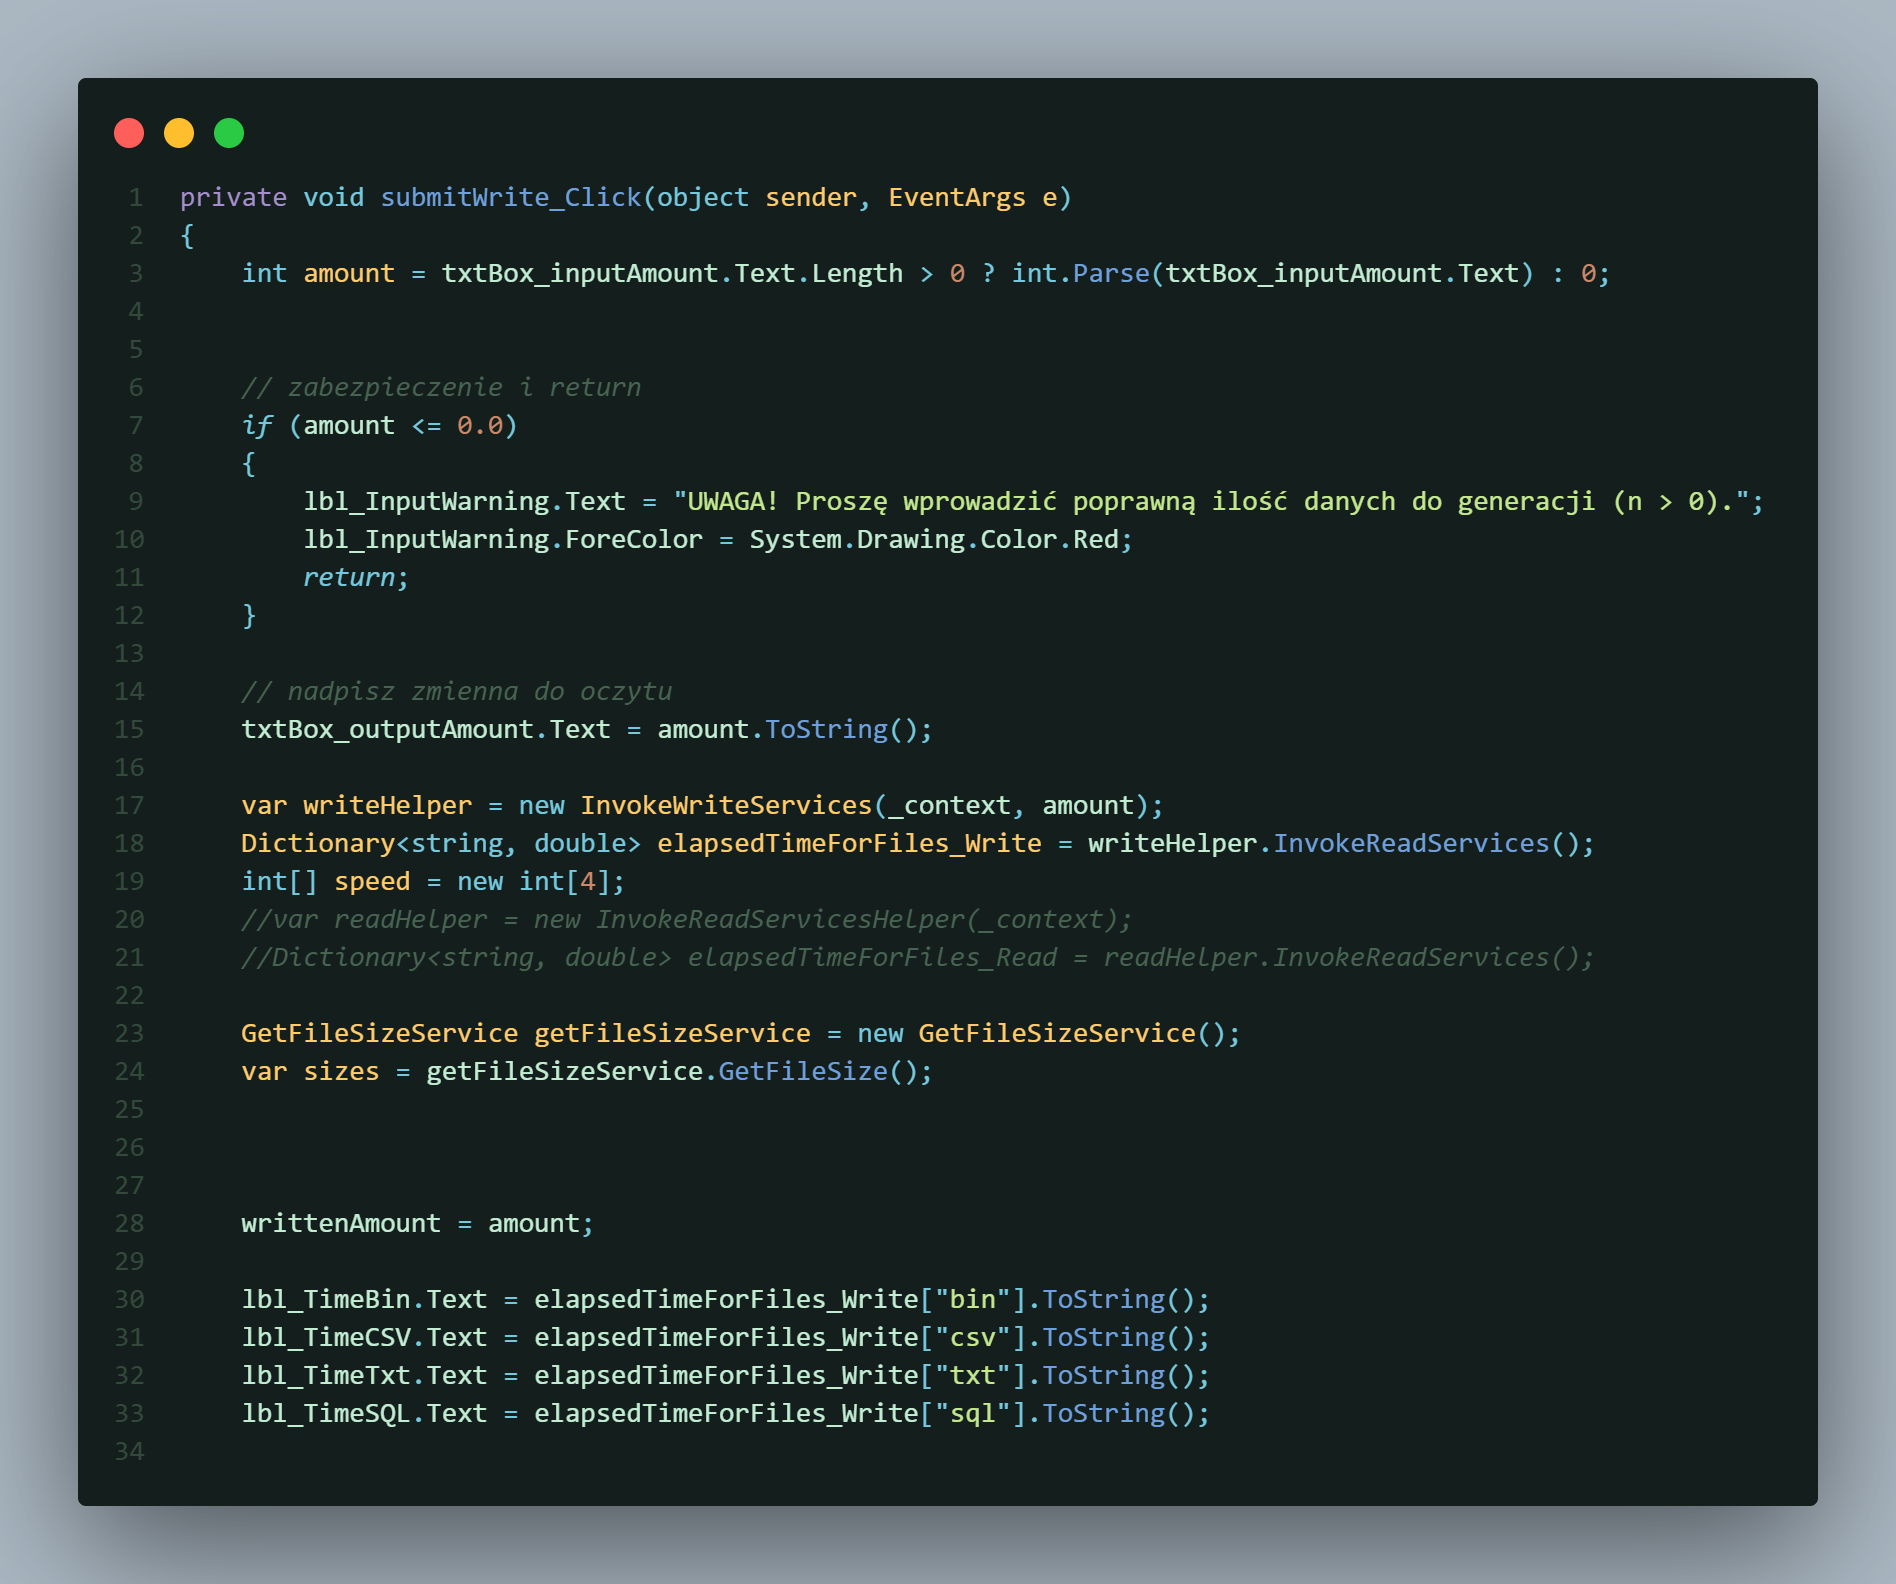
\includegraphics[width=1.0\textwidth]{src/code-ui.png}
    \caption{Fragment kodu przedstawiający implementację obsługi zdarzeń na interfejsie użytkownika}
\end{figure}

\subsection{\Large Implementacja metod zapisu do pliku}

Wszystkie metody odpowiedzialne za zapis do pliku tekstowego są do siebie bardzo podobne. Pierwszym krokiem jest wybranie odpowiedniej ścieżki, w której plik zostanie zapisany. W języku C\# można wykorzystać klasę \textit{Environment}, co umożliwia tworzenie dynamicznych ścieżek zależnych od systemu operacyjnego użytkownika.

Kolejny etap to wygenerowanie odpowiedniej ilości rekordów. Dane są generowane za pomocą biblioteki \textit{Bogus}, która pozwala na generowanie realistycznie wyglądających danych testowych, co znacząco ułatwia testowanie aplikacji.

Zasadnicza różnica między klasami obsługującymi zapis do plików różnych typów dotyczy jedynie metody samego zapisu. Dla plików binarnych używana jest klasa \textit{BinaryWriter}, natomiast dla plików tekstowych i CSV stosuje się klasę \textit{StreamWriter}. Dzięki temu każda metoda zapisu jest dostosowana do specyfiki odpowiedniego formatu pliku.

\begin{figure}
    \centering
    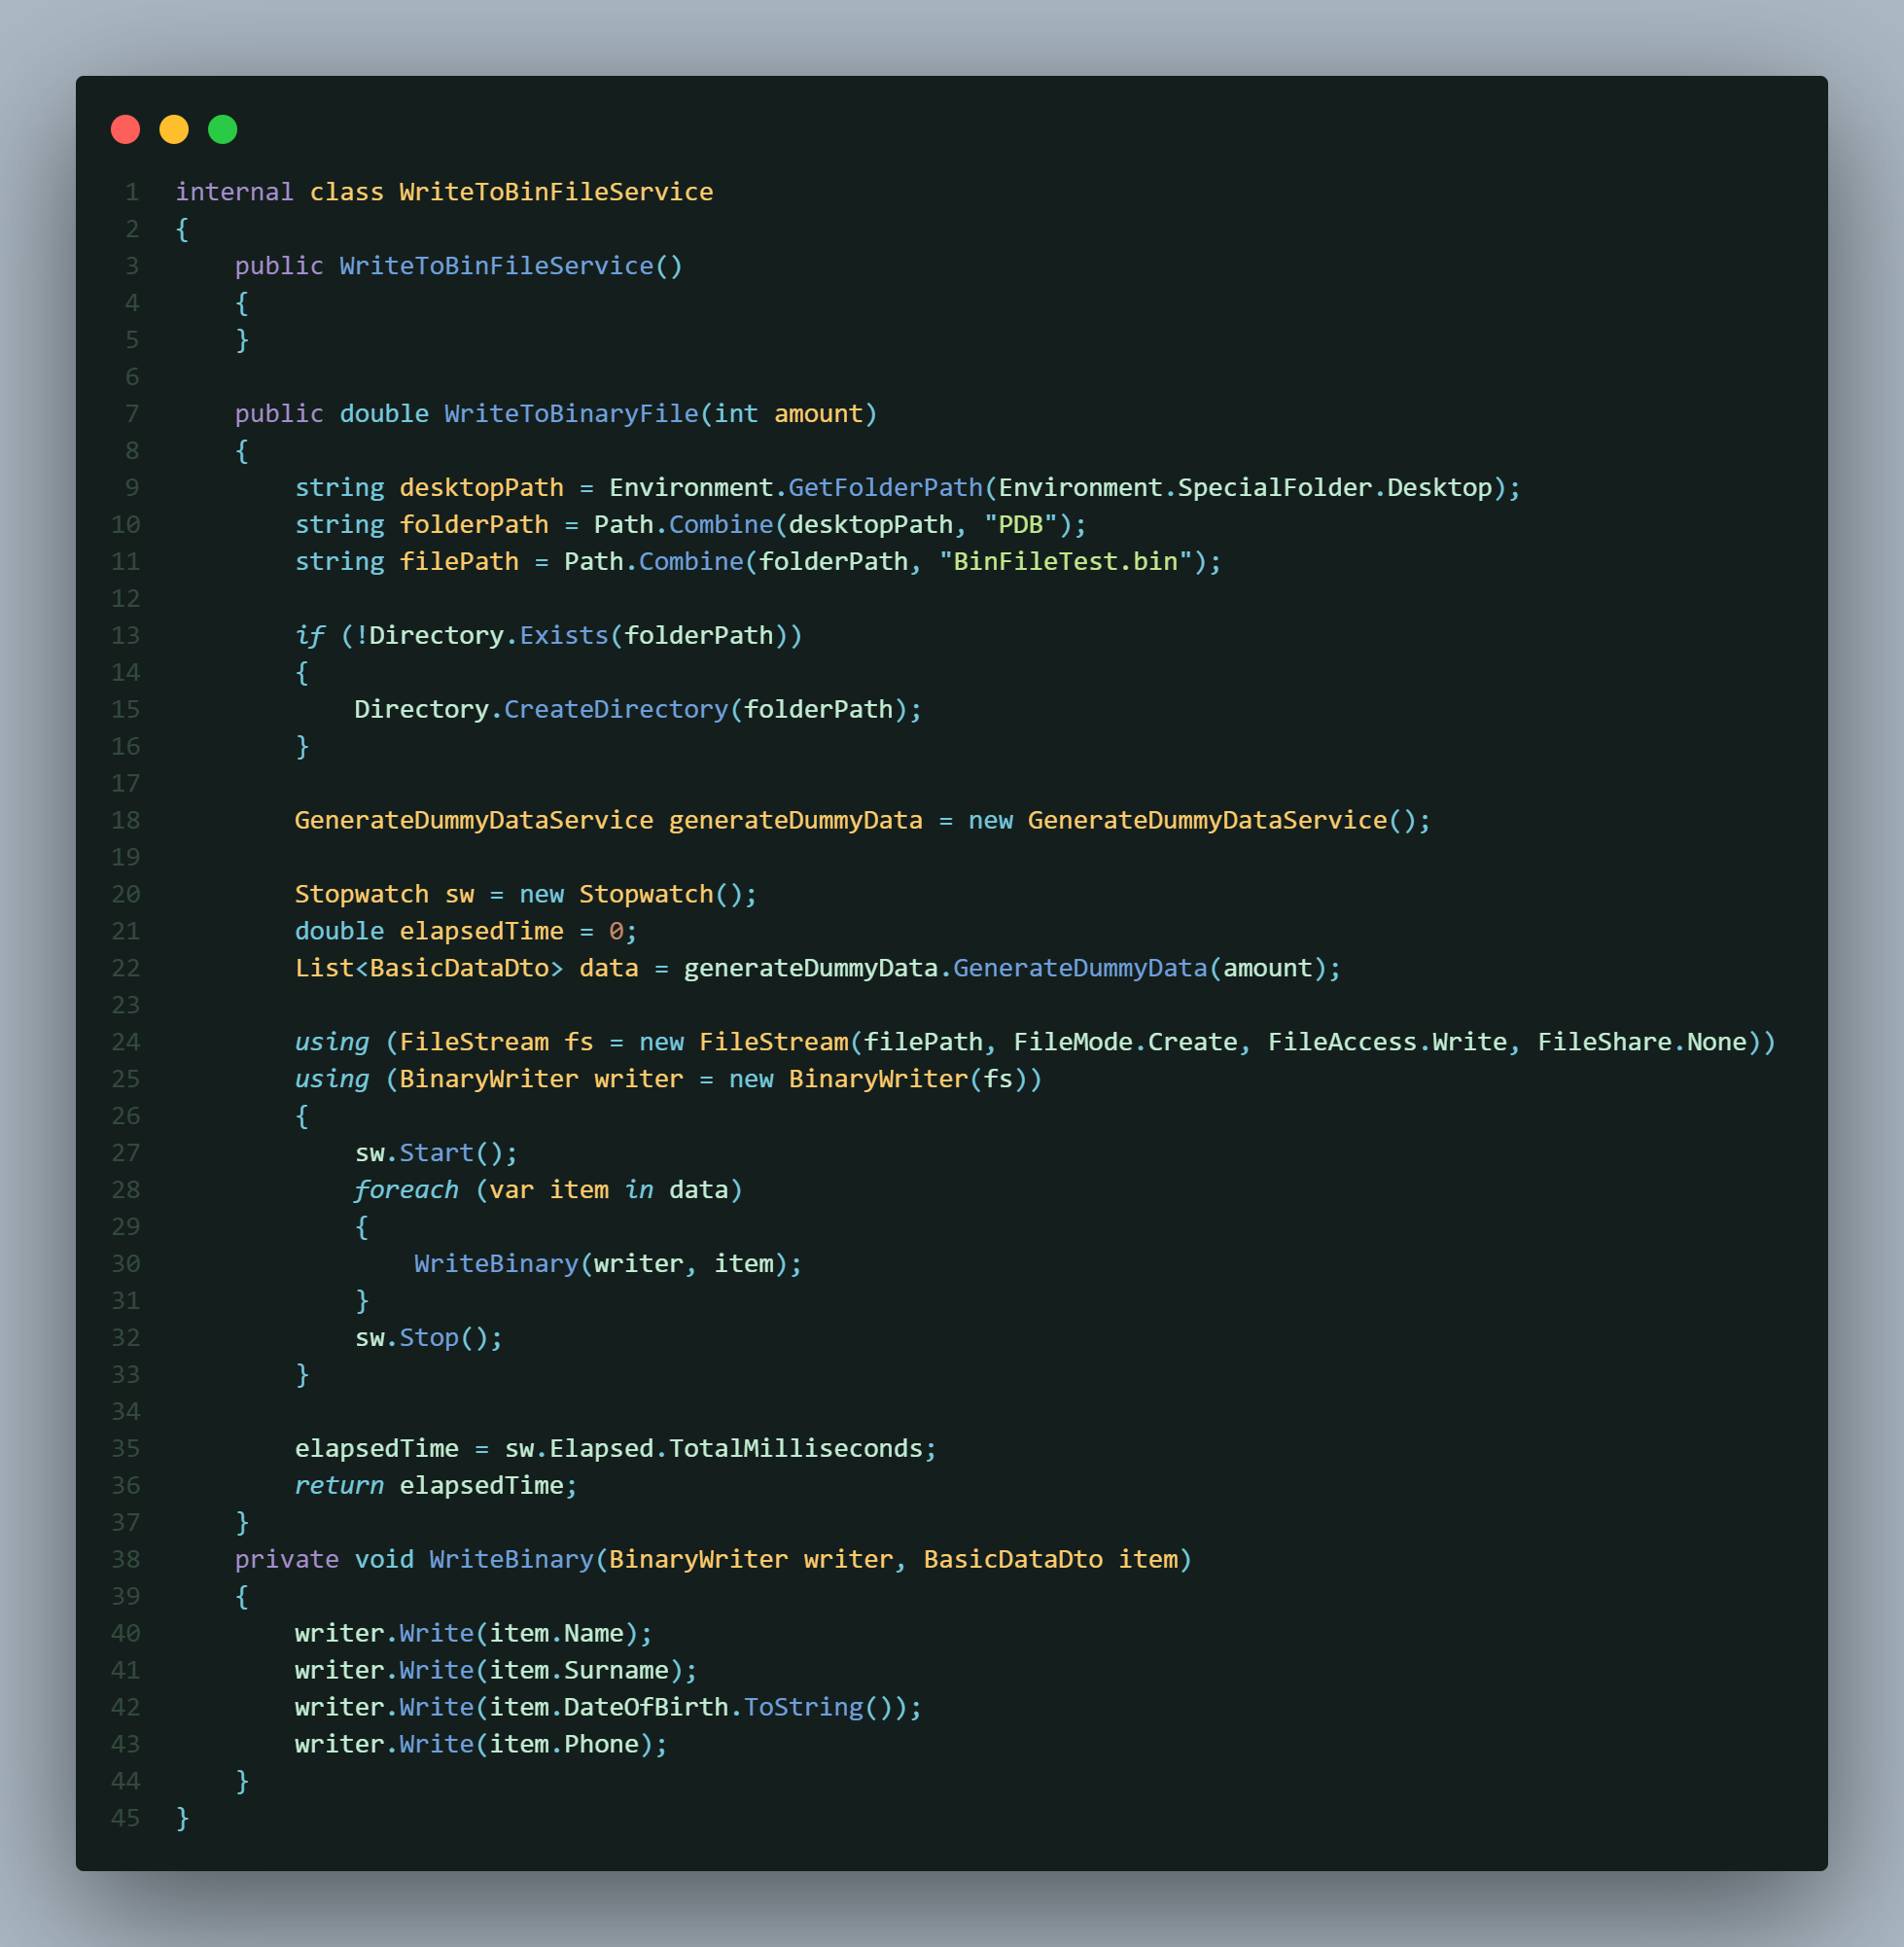
\includegraphics[width=1.0\textwidth]{src/write-bin.png}
    \caption{Klasa realizująca zapis do pliku w formacie binarnym}
\end{figure}

\subsection{\Large Implementacja zapisu do bazy danych}

Proces zapisu do bazy danych wymagał zainstalowania odpowiednich paczek, aby umożliwić korzystanie z \textit{Entity Framework}. Wymagane paczki to: 
\begin{itemize} 
    \item \textit{Microsoft.EntityFrameworkCore} 
    \item \textit{Microsoft.EntityFrameworkCore.SqlServer} 
    \item \textit{Microsoft.EntityFrameworkCore.Tools} 
\end{itemize}

Dodatkowo, do przeprowadzenia migracji, czyli sposobu, w jaki \textit{Entity Framework} zarządza zmianami w strukturze bazy danych, konieczne było upewnienie się, że pakiet \textit{.NET CLI} jest zainstalowany.

Pierwszym krokiem integracji aplikacji z bazą danych było stworzenie modelu danych. W omawianej aplikacji model ten jest reprezentowany przez klasę \textit{BasicDataDto.cs}, która odpowiada encji bazodanowej. Następnie, w celu skonfigurowania modelu, konieczne było nadpisanie metody \textit{OnModelCreating()} w klasie dziedziczącej po \textit{DbContext}. Taki zabieg informuje \textit{Entity Framework}, że dana klasa odpowiada za konfigurację struktury bazy danych.

\begin{figure}[H]
    \centering
    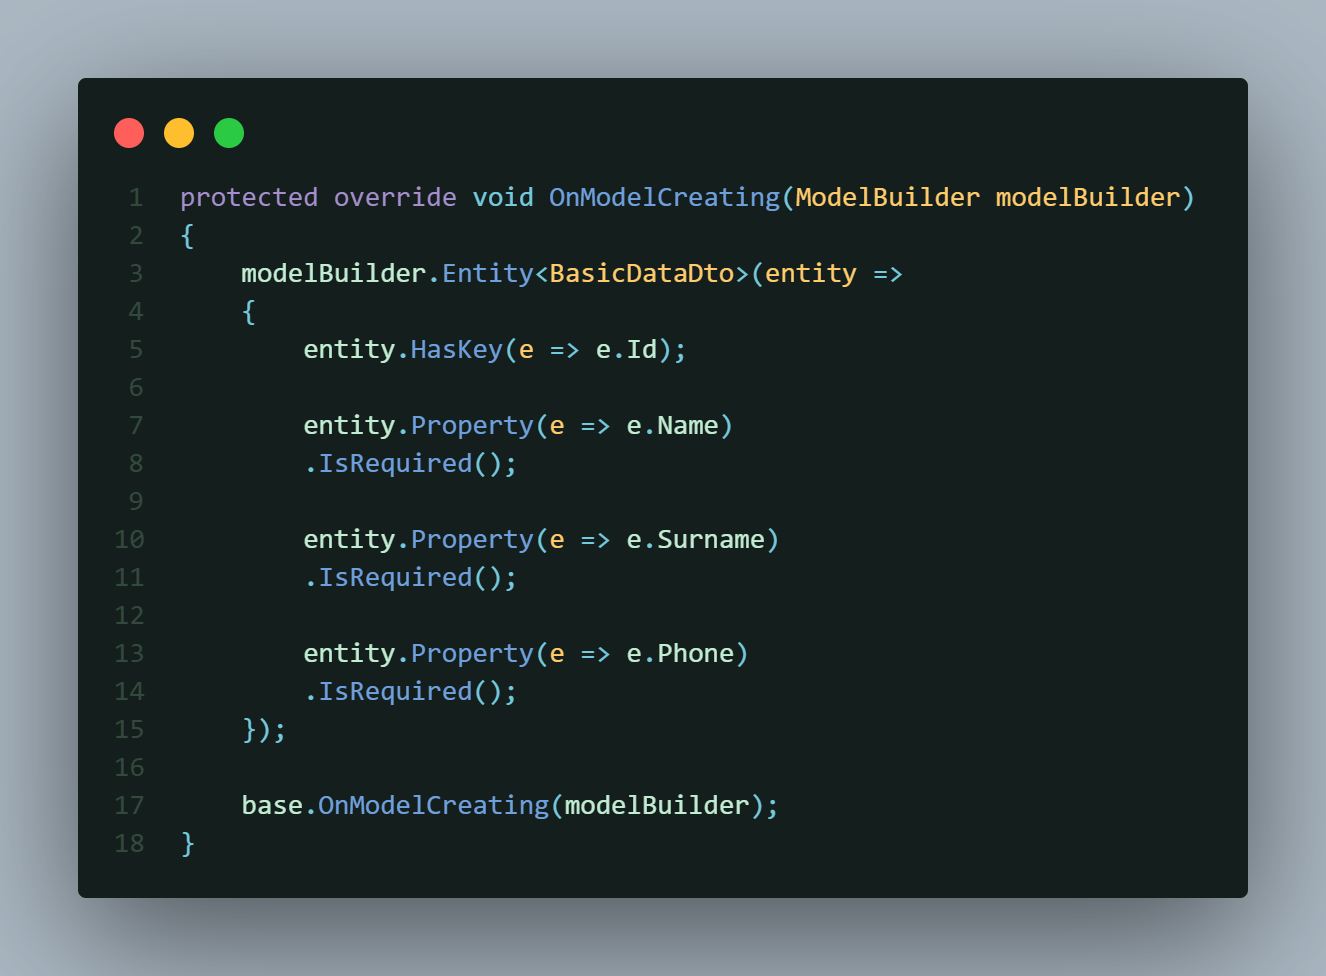
\includegraphics[width=0.8\textwidth]{src/app_dbcontext.png}
    \caption{Metoda dziedziczona po klasie DbContext, nadpisywana w klasie AppDbContext, konfigurująca encje bazy danych}
\end{figure}

Aby aplikacja mogła komunikować się z bazą danych, musiała zostać uruchomiona wewnątrz klauzuli \textit{using} w funkcji \textit{Main()}, co zapewnia odpowiednie zarządzanie połączeniami z bazą podczas działania programu.

\begin{figure}[H]
    \centering
    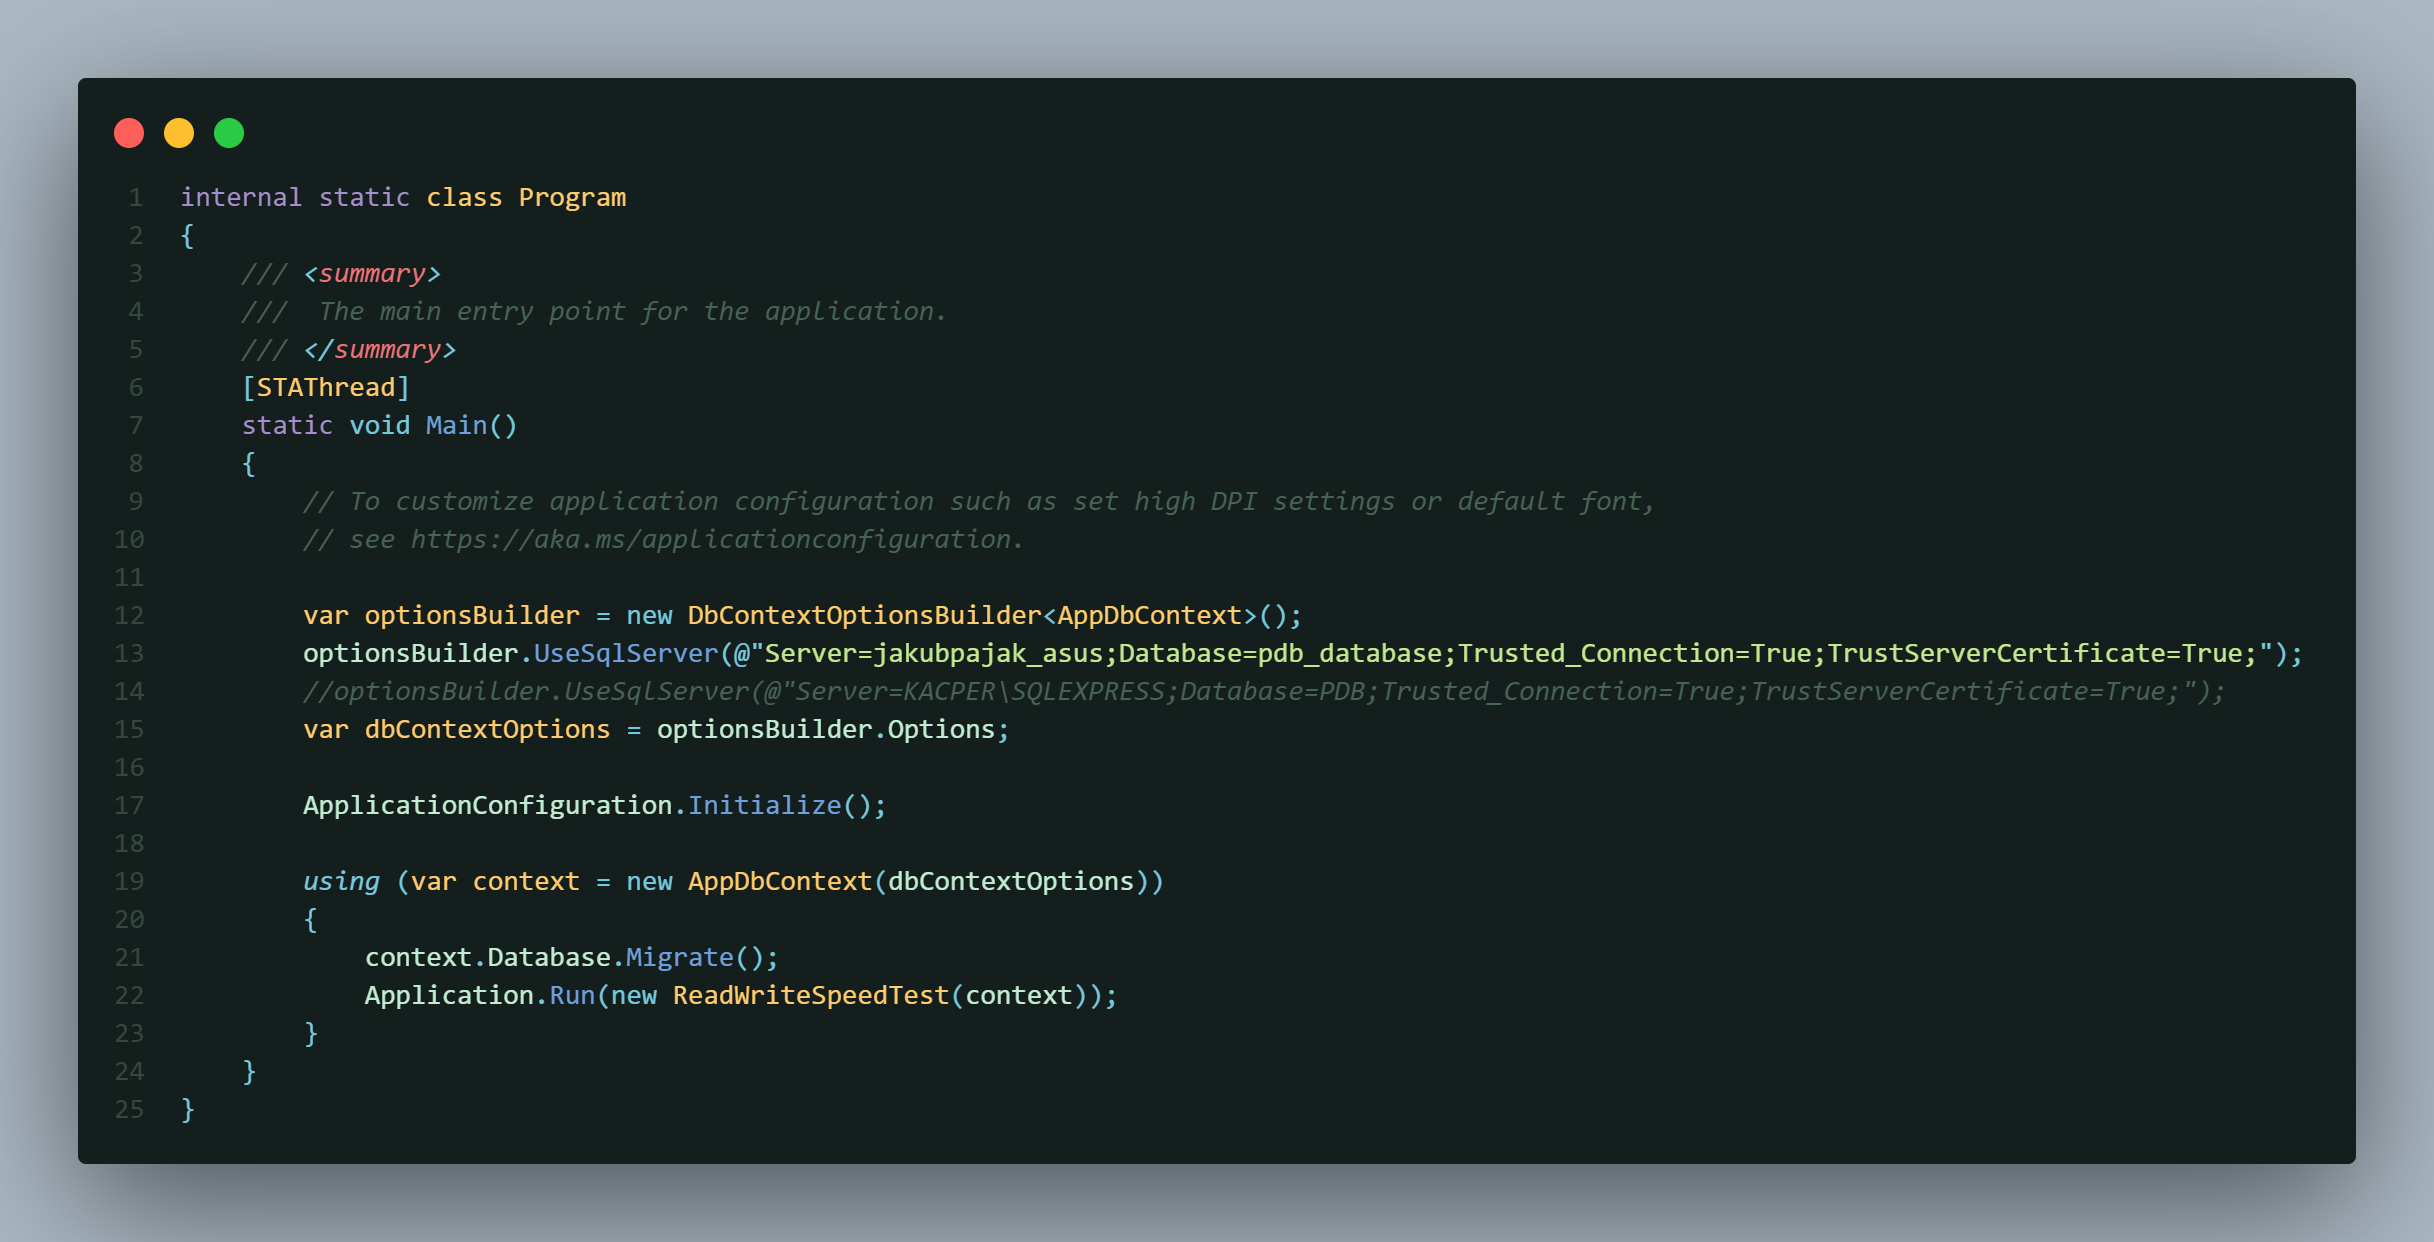
\includegraphics[width=1.0\textwidth]{src/main.png}
    \caption{Klasa będąca punktem startowym aplikacji. Znajduje się w niej uruchomienie aplikacji oraz wywołanie metody aktualizującej migracje}
\end{figure}

Sam proces zapisu danych do bazy jest stosunkowo prosty. Do kontekstu bazy danych dodawane są nowe rekordy, po czym metoda \textit{SaveChanges()} zapisuje zmiany w bazie danych, zapewniając trwałość operacji.

\begin{figure}[H]
    \centering
    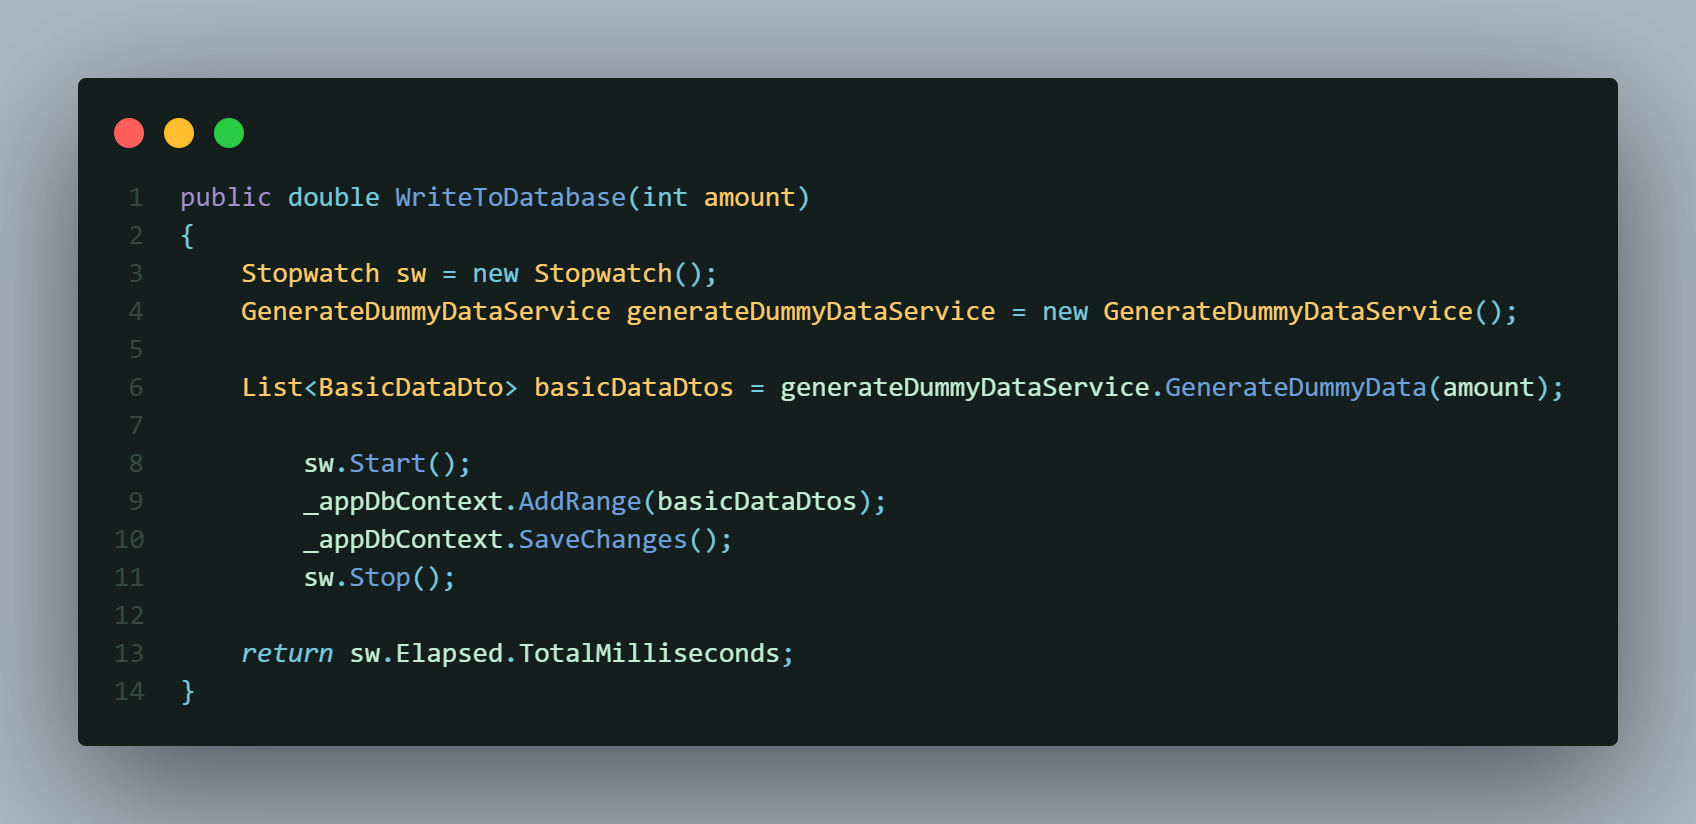
\includegraphics[width=1.0\textwidth]{src/db_write.png}
    \caption{Metoda odpowiadająca za zapis rekordów do bazy danych}
\end{figure}

\subsection{\Large Implementacja metod odczytu z pliku}

Implementacja metod odczytu z pliku we wszystkich metodach przebiega bardzo podobnie. Pierwszym etapem jest utworzenie ścieżki do pliku za pomocą klasy \textit{Environment}. Następnie tworzona jest instancja klasy \textit{Stopwatch} w celu pomiaru czasu potrzebnego do odczytania danych. Kolejnymm krokiem jest właściwy odczyt z pliku, realizowany wewnątrz struktury \textit{try-catch}. W przypadku odczytu z pliku binarnego skorzystano z klasy \textit{BinaryReader}. W pozostałych klasach odczytujących z pliku tekstowego oraz CSV, wykorzystano klasę \textit{StreamReader}. 

\begin{figure}[H]
    \centering
    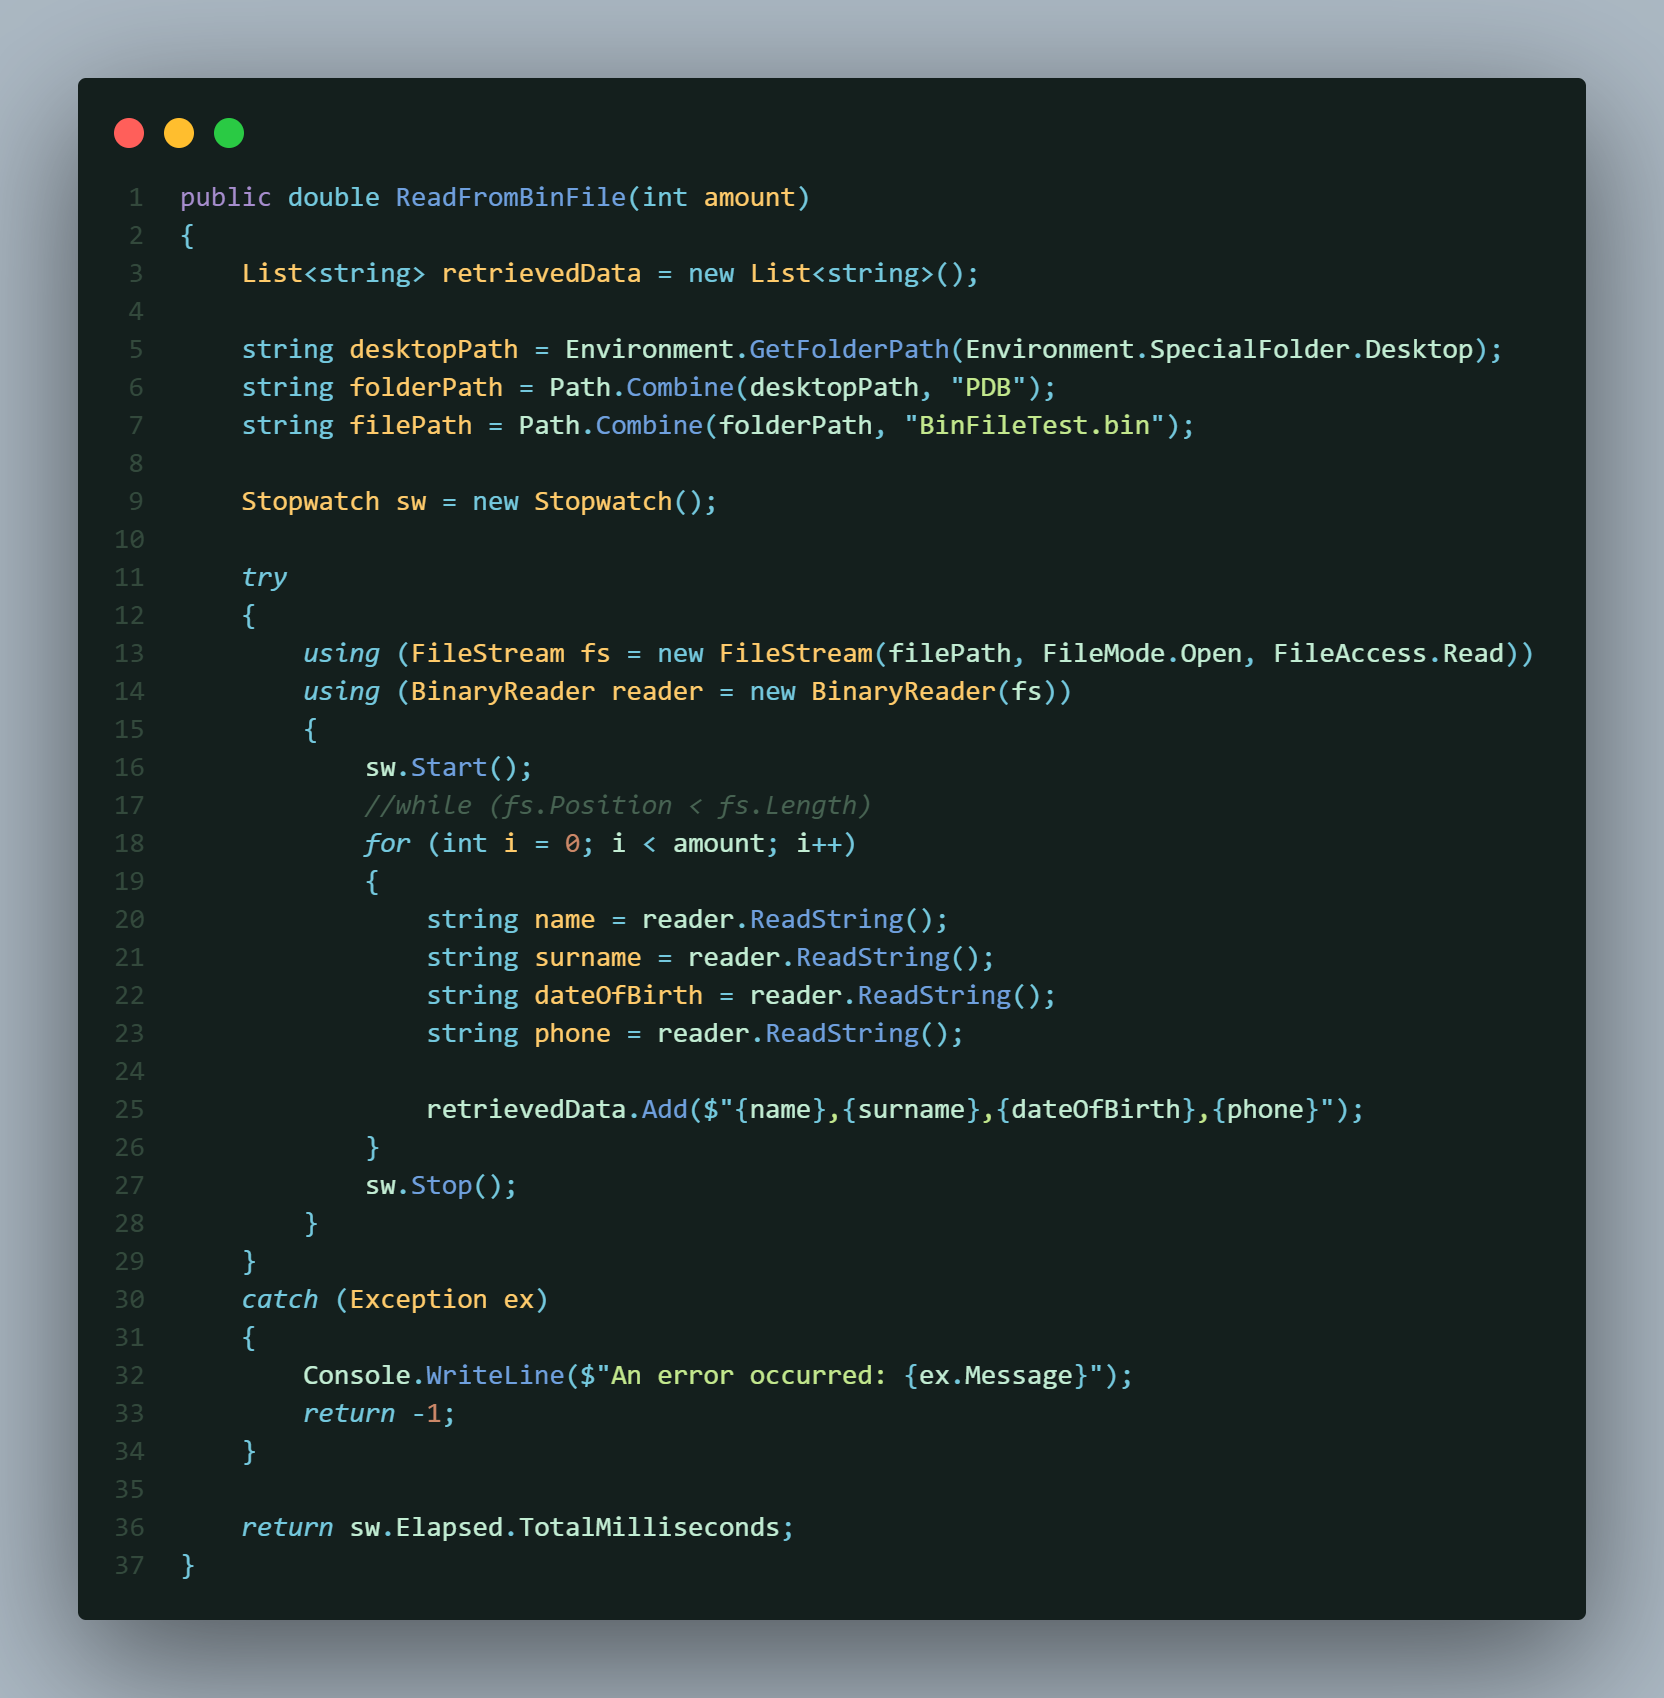
\includegraphics[width=1.0\textwidth]{src/bin-read.png}
    \caption{Metoda odpowiadająca za odczyt rekordów z pliku binarnego}
\end{figure}

\begin{figure}[H]
    \centering
    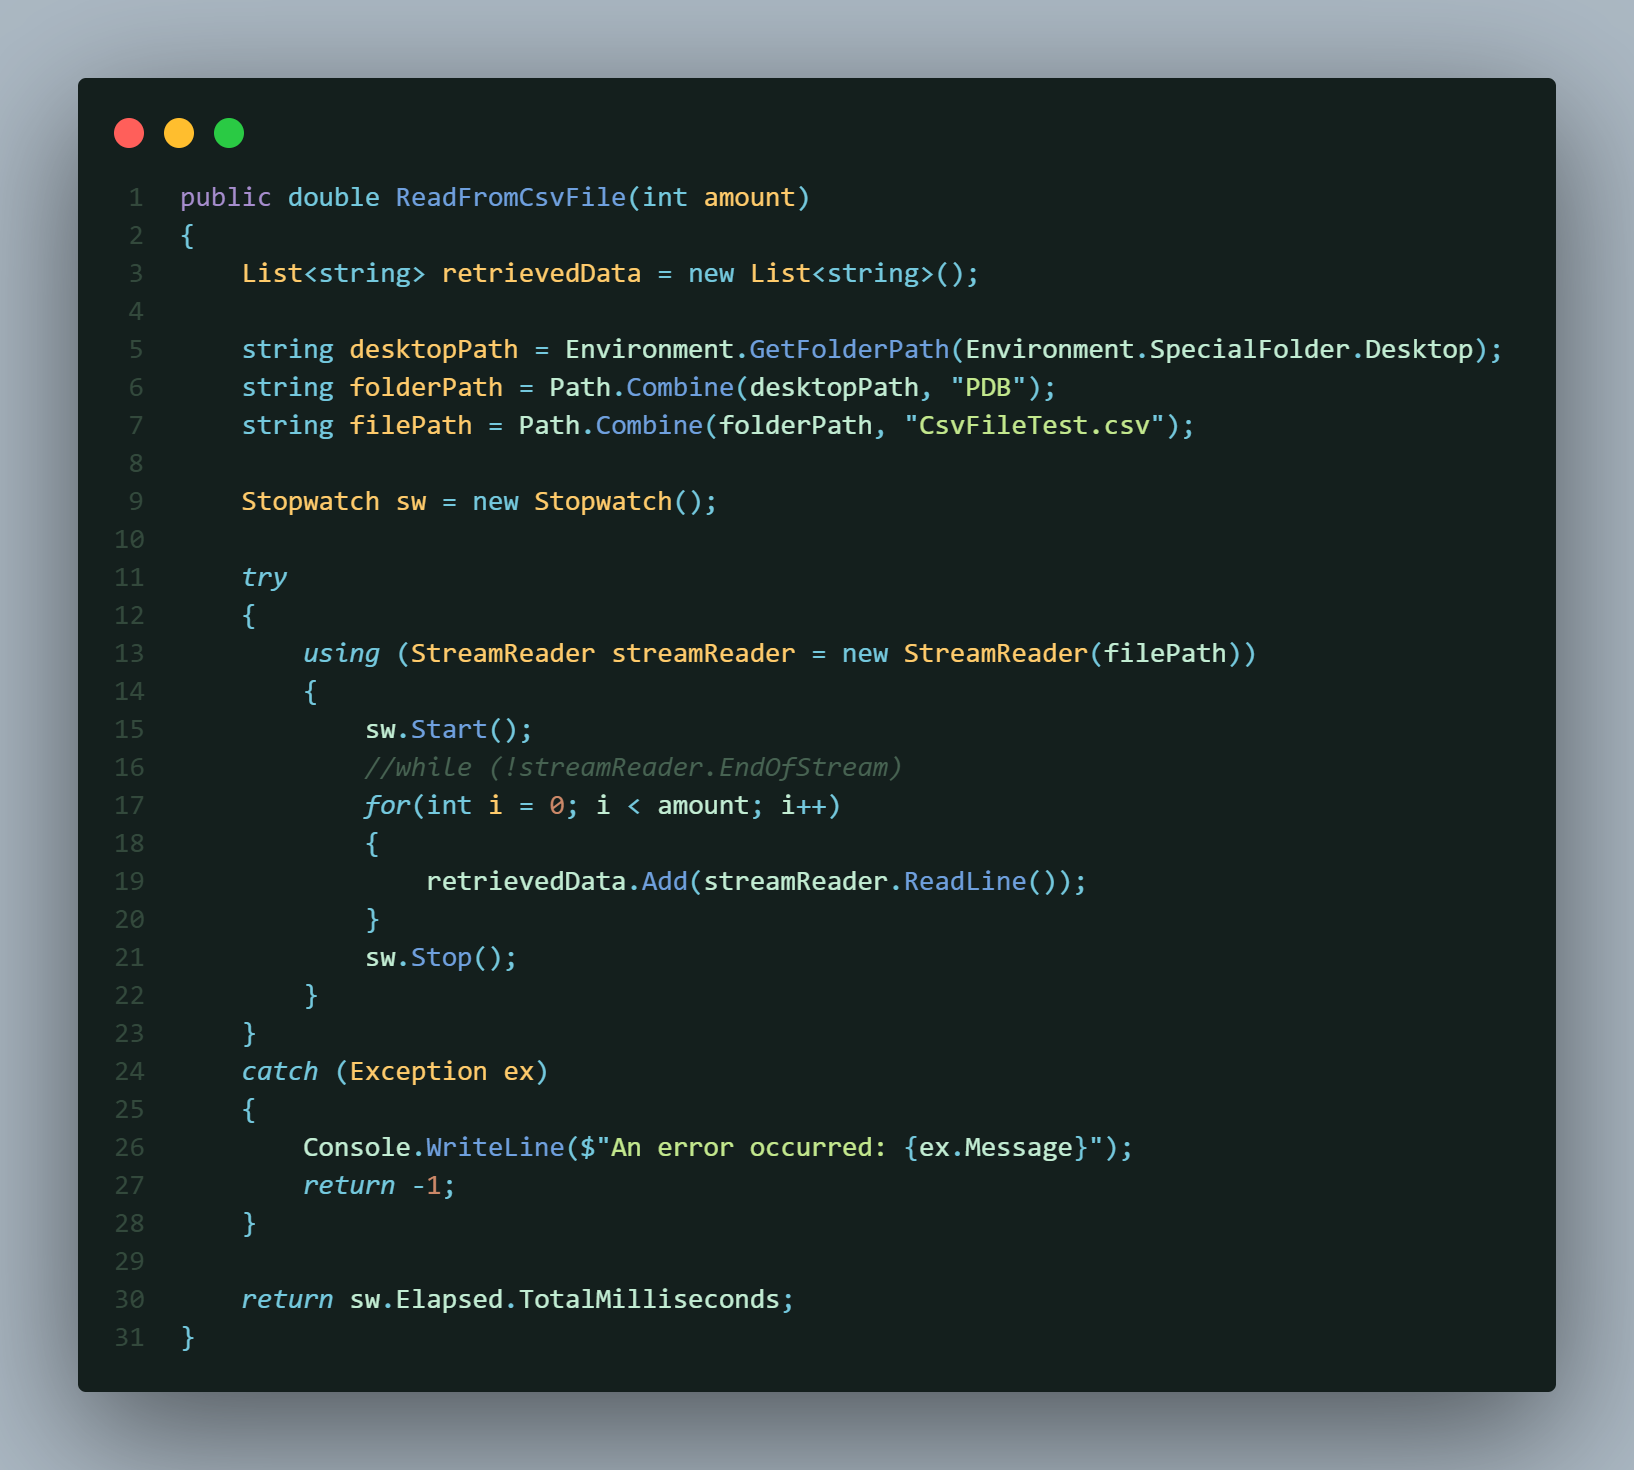
\includegraphics[width=1.0\textwidth]{src/csv-read.png}
    \caption{Metoda odpowiadająca za odczyt rekordów z pliku CSV}
\end{figure}

\subsection{\Large Implementacja odczytu danych z bazy danych}

Implementacja odczytu rekordów z bazy danych jest prosta - opiera się na wykorzystaniu metody \textit{Take()} wywołanej na obiekcie kontekstu bazy danych. Jednoczenie uwidacznia to wielką zaletę korzystania z EF - programista nie musi korzytać bezpośrednio z zapytań SQL, tylko wprost z języka C\# oraz wyrażeń \textit{lambda} i metod udostępnionych na obiekcie DbContext. 

\begin{figure}[H]
    \centering
    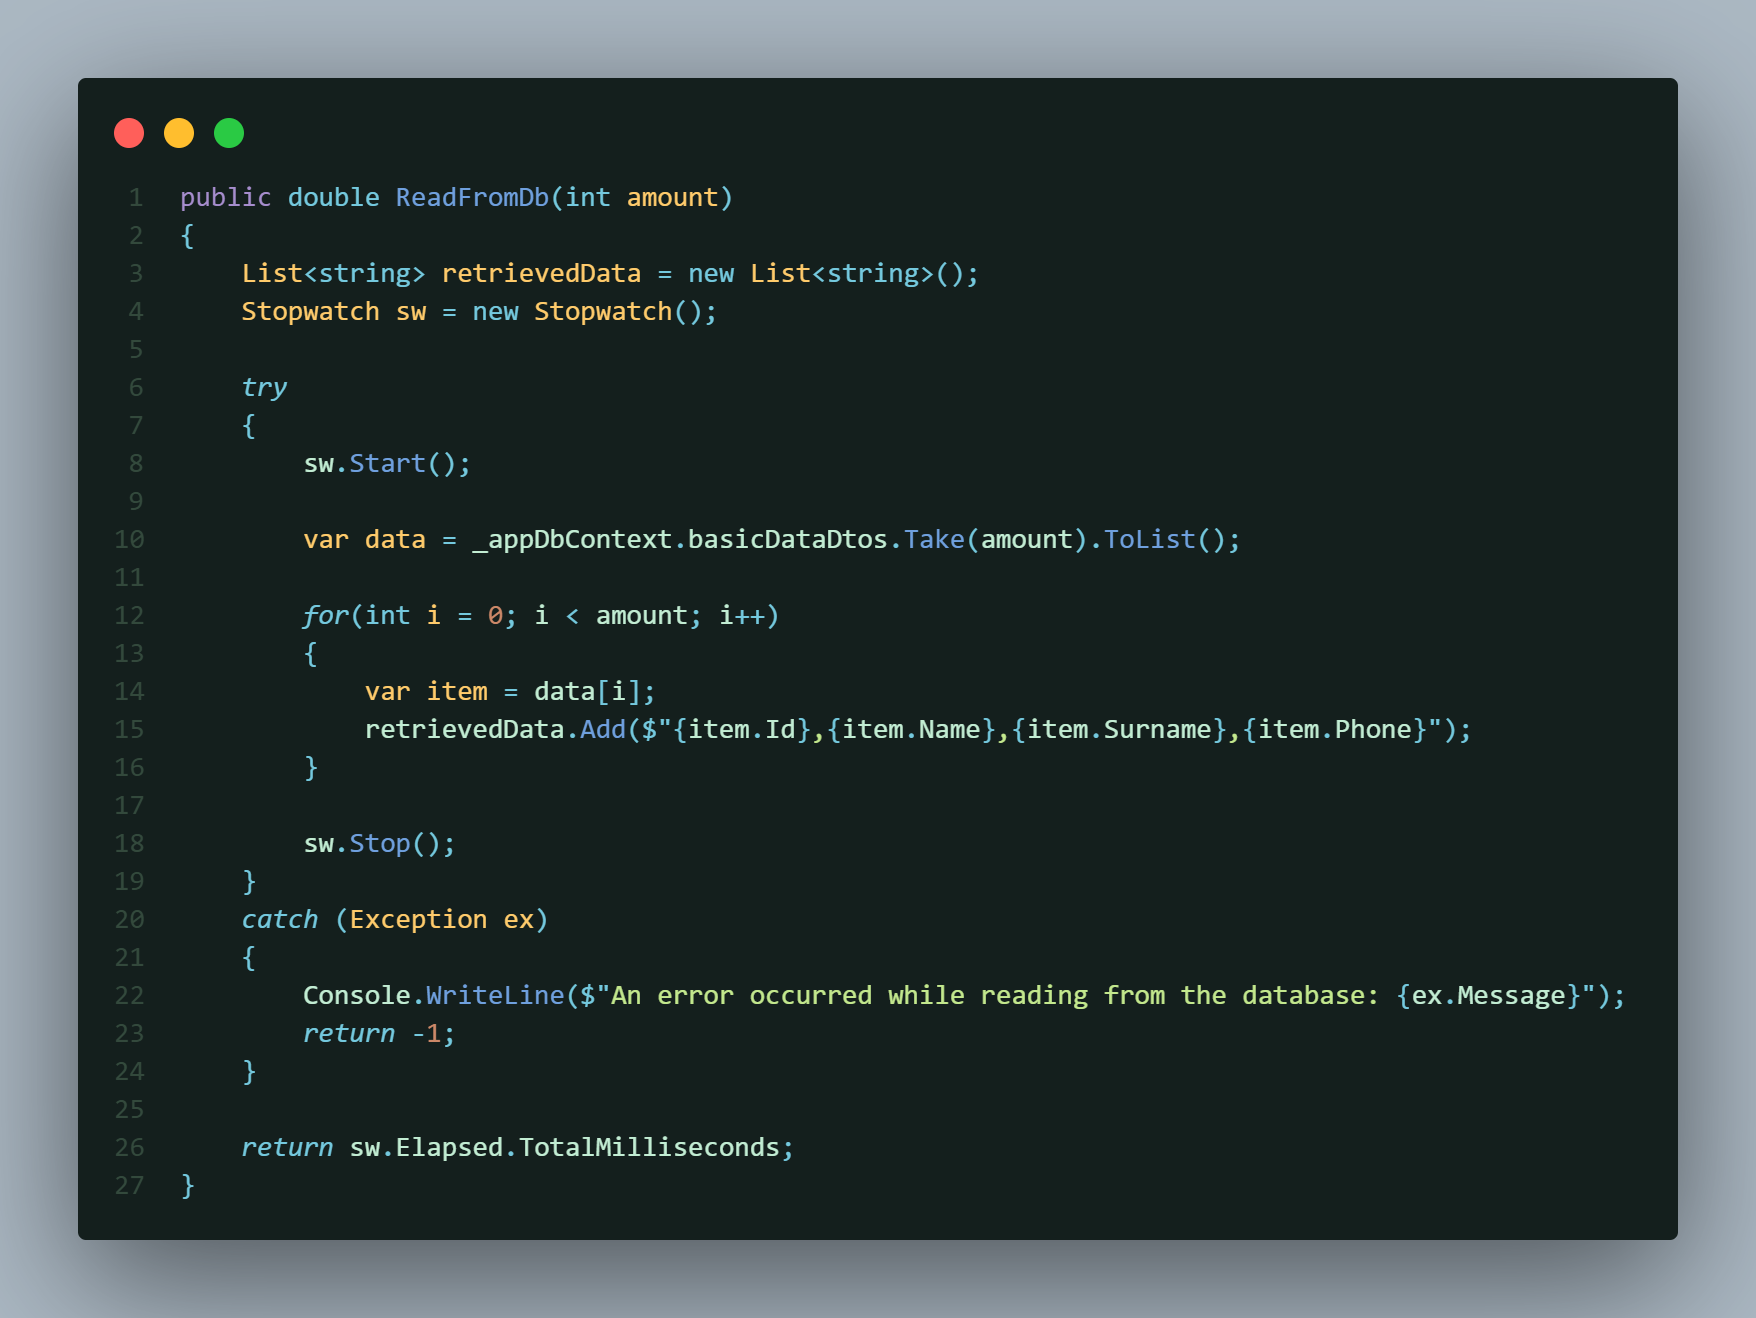
\includegraphics[width=1.0\textwidth]{src/db-read.png}
    \caption{Metoda odpowiadająca za odczyt rekordów z bazy danych}
\end{figure}

\section{Działanie aplikacji}
\subsection{Generacja pliku wsadowego oraz jego zapis}
Użytkownik po uruchomieniu aplikacji może wygenerować plik o określonej przez niego długości rekordów a następnie dokoknuje się zapis pliku w formacie .txt, .bin, .csv oraz bazodanowy.

\begin{figure}[h]
\centering
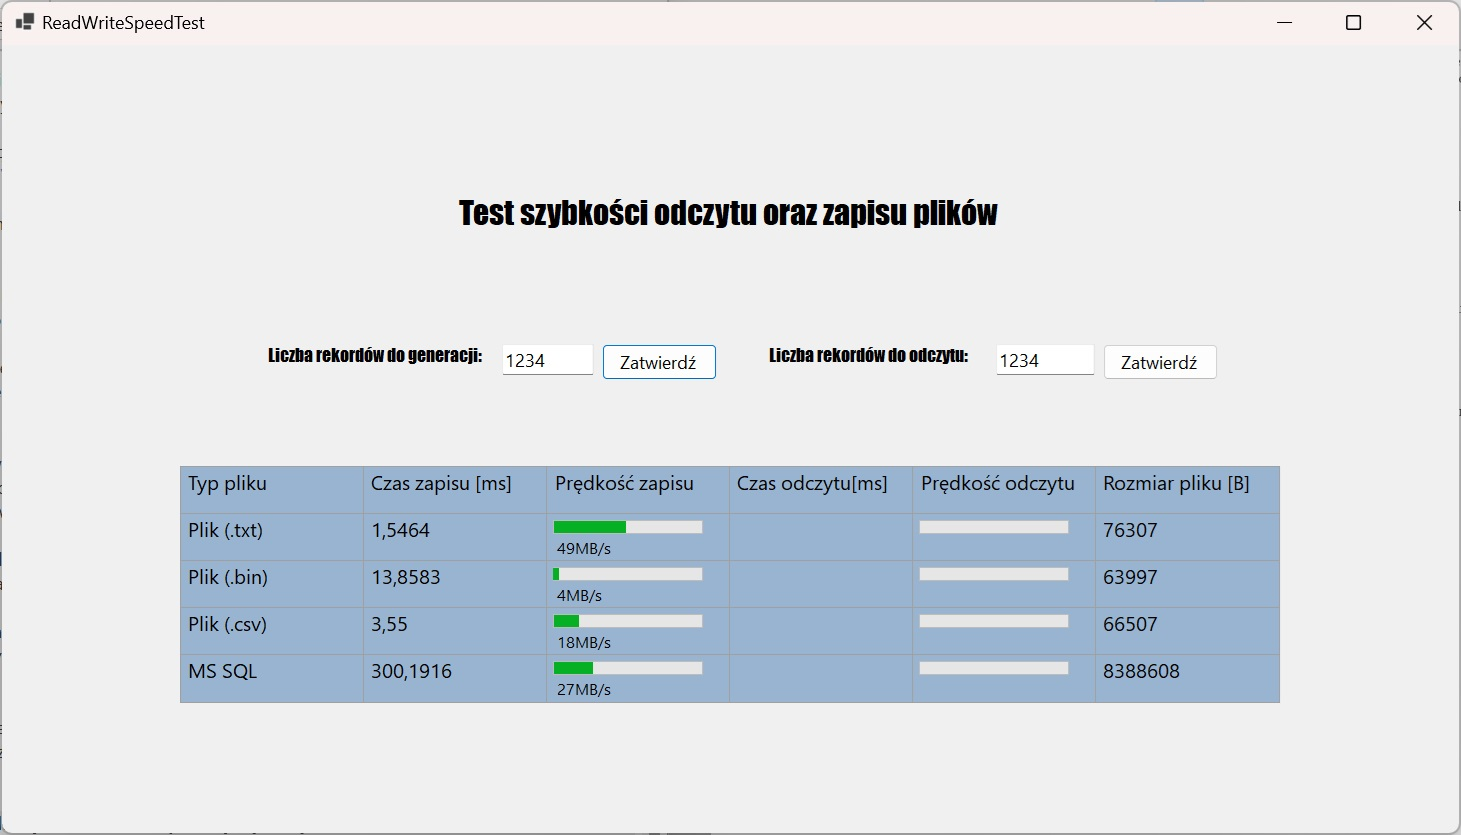
\includegraphics[width=15cm]{img/zapis.jpg}
\caption{Zapis plików}
\end{figure}

\subsection{Odczyt pliku}
Po zapisaniu plików można przejść do kolejnego okienka, w którym należy podać ilość rekordów z pliku do odczytu. Automatycznie przepisywana jest wartość określona przy zapisie lecz użytkownik może dowolnie zmienić tą ilość.

\begin{figure}[h]
\centering
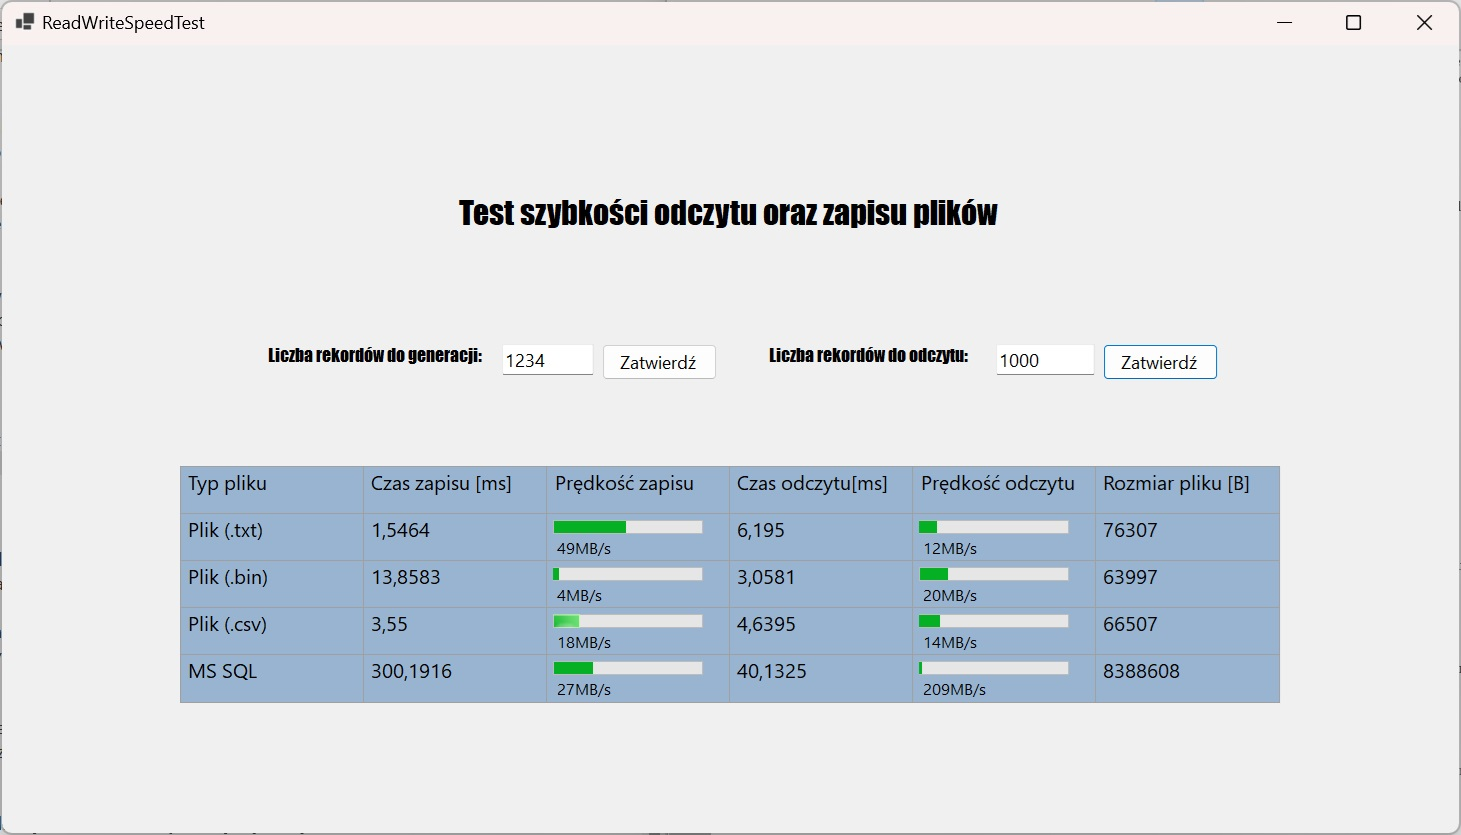
\includegraphics[width=15cm]{img/odczyt.jpg}
\caption{Odczyt plików}
\end{figure}

\subsection{Wizualizacja danych}
W tabeli poniżej okienek do wprowadzania wartości po zapisie i odczycie aktualizowana jest tabela z właściwościami: czasu zapisu i odczytu w milisekundach, prędkości zapisu i odczytu w MB/s oraz rozmiarem pliku w bajtach. Dodatkowo paski obrazujące prędkość zapisu skalują się wraz z rosnącą wartością prędkości, aby uniknąć błędów programu.

\begin{figure}[h]
\centering
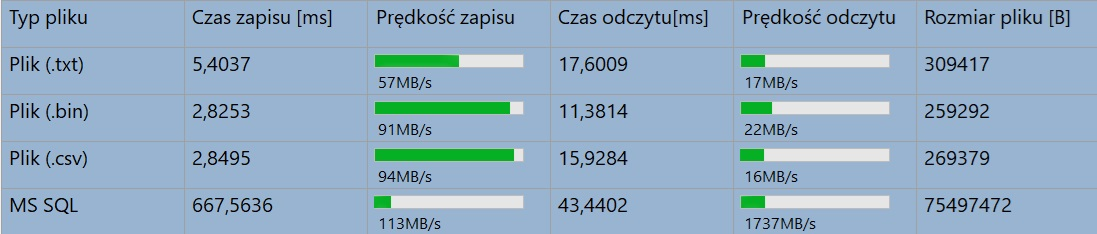
\includegraphics[width=15cm]{img/tab.jpg}
\caption{Tabela danych}
\end{figure}

\subsection{Zabezpieczenia}
Aplikacja posiada zabezpiczenia przed wpisaniem ujemnej wartości rekrodów oraz przed wybraniem do odczytu większej ilości rekordów niż zostały zapisane, co mogłoby powodować poważne usterki programu. Jak w akapicie wyżej, zastosowano także zabepieczenie przed przepełnieniem wartości wizualizowanej przez paski postępu.

\begin{figure}[H]
\centering
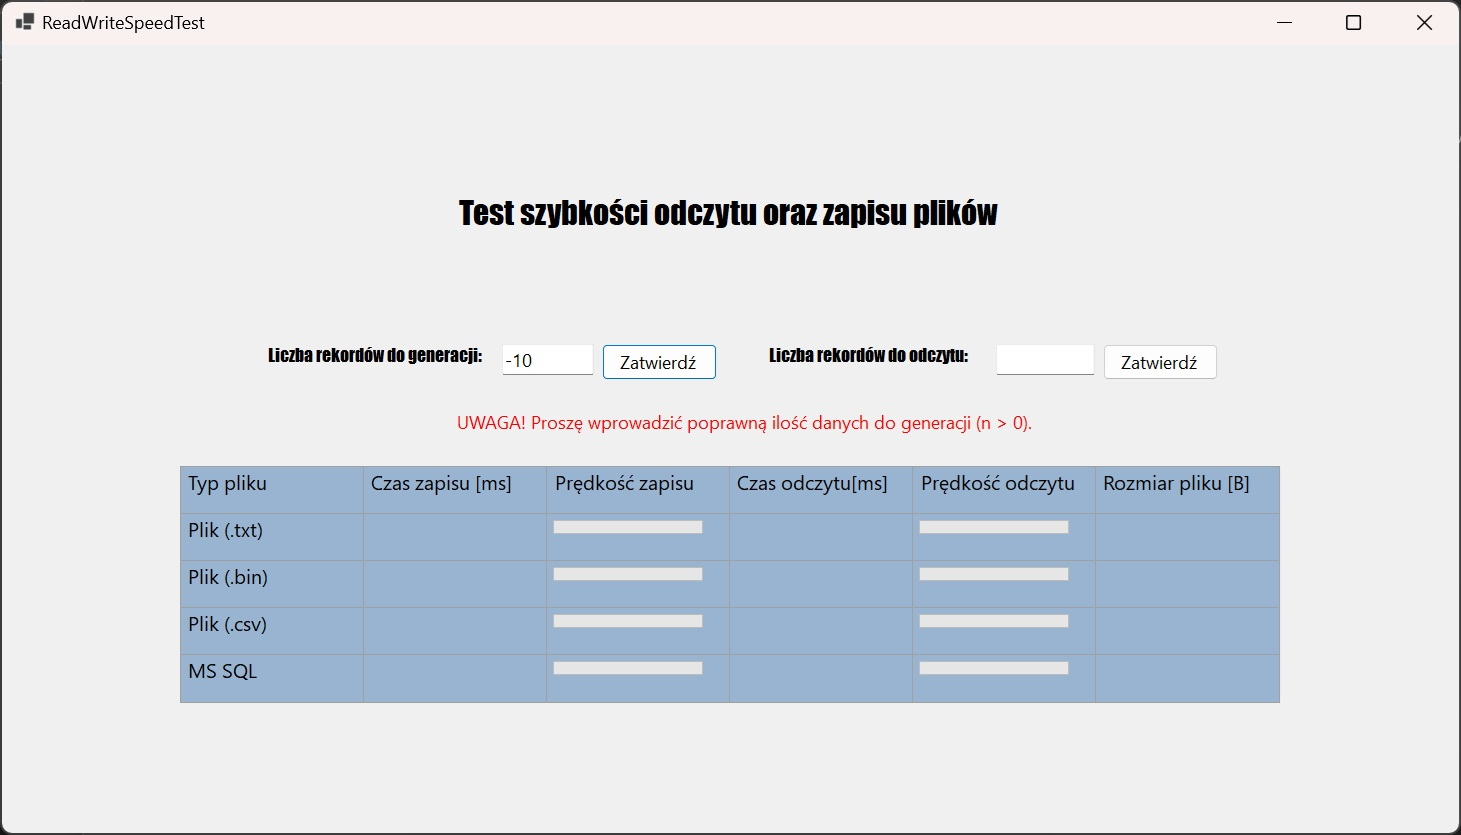
\includegraphics[width=15cm]{img/zapis_error.jpg}
\caption{Błąd zapisu}
\end{figure}

\begin{figure}[H]
\centering
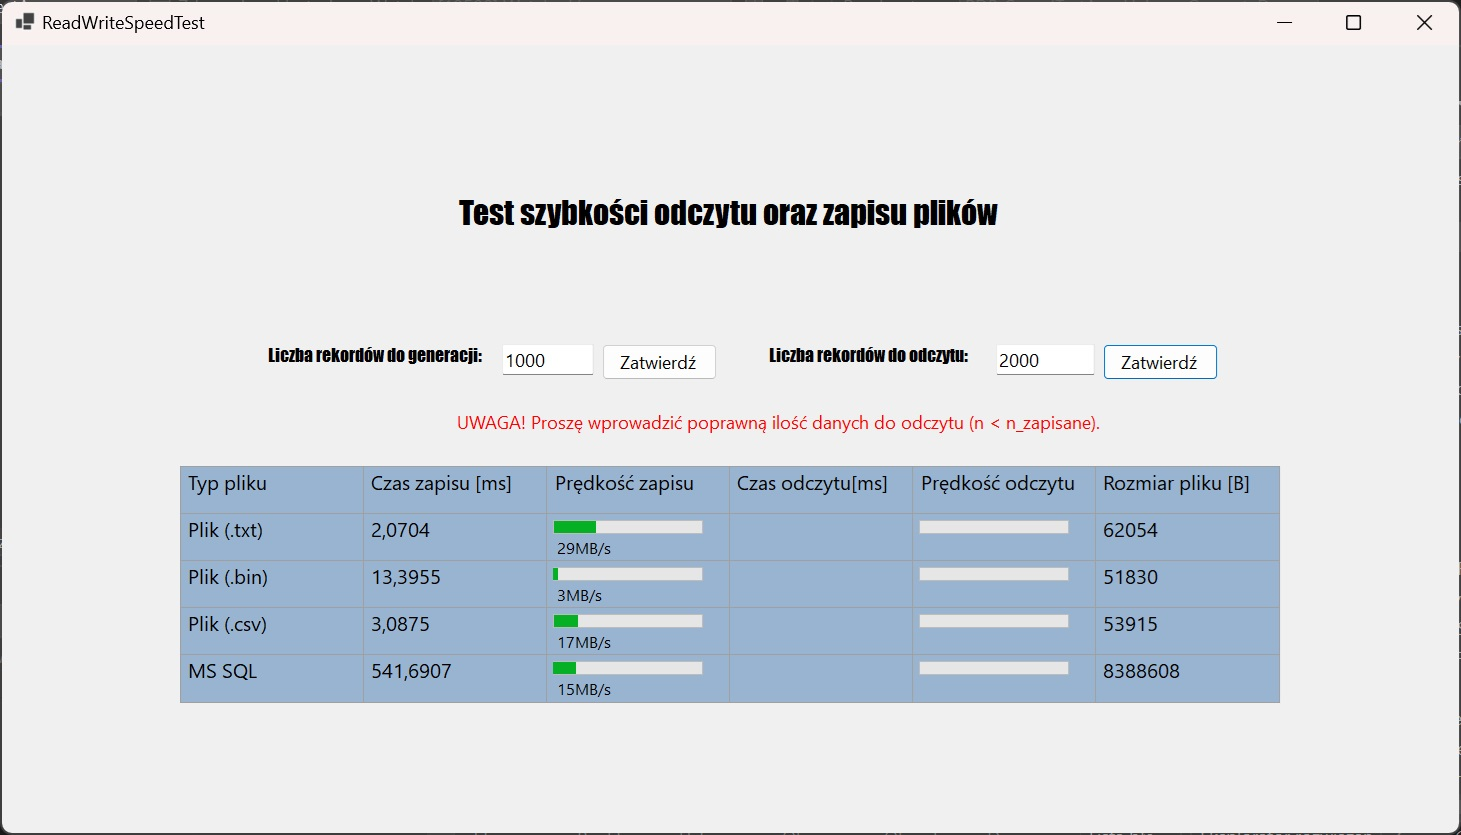
\includegraphics[width=15cm]{img/odczyt_error.jpg}
\caption{Błąd odczytu}
\end{figure}

\section{Wnioski}

Na podstawie wyników uzyskanych podczas testów szybkości zapisu danych do różnych typów plików oraz bazy danych stwierdzono, że zapis do bazy danych wymaga najwięcej czasu. Najszybszy okazał się zapis do pliku binarnego, jednak różnice między nim a plikiem tekstowym oraz CSV są niewielkie i wynoszą około 2 ms przy dużych zbiorach danych. Wraz ze zmniejszaniem się liczby danych różnice te stają się mniej istotne.

Odczyt danych wykazał podobne zależności. Istnieje bardziej wyraźna różnica między czasem odczytu z pliku binarnego a innymi typami plików, jednak odczyt z bazy danych okazuje się szybszy, co częściowo zmniejsza tę różnicę. Niemniej jednak, baza danych nadal charakteryzuje się istotnie dłuższym czasem operacji w porównaniu z pozostałymi metodami.

\begin{figure}[H]
\centering
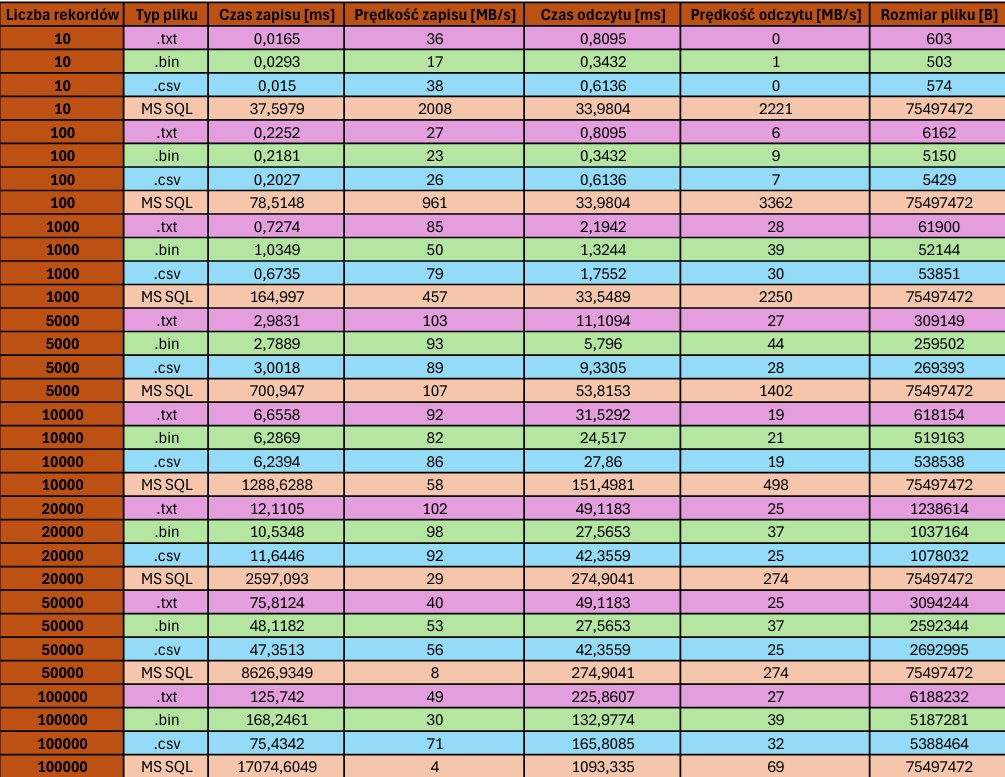
\includegraphics[width=15cm]{img/tabela-porwn.jpg}
\caption{Porownanie}
\end{figure}

\end{document}